\subsubsection{Evaluation verfügbarer Produkte}
\label{sec:product-evaluation}

\paragraph{Auswahl der \ac{waf}-Anwendung}\ \\

Das Herzstück der Laborumgebung ist die \ac{waf} Anwendung.
Mit dieser interagieren die Lernenden in der Laborumgebung am meisten.
Sie wird nach einigen Kriterien Bewertet:
\begin{description}
    \item[Bedienbarkeit:] Um den Fokus auf den \ac{waf}-Regeln legen zu können sollten die Hürden zum Einstieg in die \ac{waf} möglichst gering sein
    \item[Flexibilität:] Da sich die Laborumgebung von dem gewöhnlichen Einsatzgebiet einer \ac{waf} unterscheidet, muss die gewählte Anwendung leicht anpassbar sein.
    So ist es beispielsweise notwendig das vorkonfigurierte Regelwerk, mit dem die meisten \acp{waf} ausgeliefert werden zu entfernen und eine eigenständige Konfiguration von Grund auf zu ermöglichen.
    \item[Kosten:] Da die Laborumgebung in de Lehre eingesetzt werden können muss dürfen nahezu keine Kosten entstehen.
    \item[Debugging:] Da die Lernenden die \ac{waf}-Regeln voraussichtlich nicht direkt fehlerfrei erstellen werden, muss ein einfacher Zugriff auf Debugging Logs möglich sein um die Funktion der erstellten Regeln analysieren können.
\end{description}

Eine unkomplizierte Möglichkeit eine Website mit einer \ac{waf} abzusichern sind die Angebote von Cloud-Providern wie \textit{CloudFlare} oder \textit{Microsoft Azure}.
Beide ermöglichen es Nutzern mittel weniger Klicks eine einfache \ac{waf} vor ihrer öffentlichen Webseite zu Platzieren.
Für Studierenden sind diese Angebote Außerdem kostenfrei nutzbar.
Jedoch bieten diese einfachen \textit{Cloud-\acp{waf}} nahezu keine Möglichkeit der Konfiguration oder Anpassbarkeit.
Deshalb eigenen sich derartige Angebote nicht für die Laborumgebung.\\

Während grundlegende Cloud-\acp{waf} wie sie oben beschreiben sind hauptsächlich für Privatnutzer bestimmt sind, werden in Industriellen und Produktiven Umgebungen eigenständige \acp{waf} genutzt.
Im Ramen stehen zur evaluation die Produkte \textit{Airlock} der Schweizer Firma \textit{Ergon} sowie die \textit{Barracuda \ac{waf}} der US Amerikanischen Firma \textit{Barracuda Networks} zur Verfügung.
Die Unterschiede der beiden Produkte liegen hauptsächlich in Performance, erweiterten Funktionen und Kosmetik.
Alles Kriterien die für die Laborumgebung nicht relevant sind.

Vorteile finden sich jedoch in der Nutzbarkeit.
Die Grafische Oberfläche ermöglicht eine flache Lernkurve und schnellen Einstieg in die kerninhalte der Laborumgebung.
Außerdem werden beide Produkte mit Log-Analyse Programmen ausgeliefert die es Nutzern mittels grafischer Interfaces ermöglicht die Logs der \ac{waf} zu analysieren.

Jedoch können diese kommerziellen Produkte in der Laborumgebung nicht sinnvoll eingesetzt werden:
Die Kosten belaufen sich auf mehrere Tausend Euro pro Instanz, die auch nur über Vertriebspartner erhalten werden könne.
Des Weiteren werden Sicherheitskritische Anwendungen wie eine \ac{waf} üblicherweise mit einem gehärteten Betriebssystem ausgeliefert.
Dadurch ist ein Zugriff auf die tieferen Ebenen der Anwendung nicht möglich.
Auch lässt sich die mitgelieferte Konfiguration nicht aus der Anwendung entfernen.
Zwar lassen sich einzelne Regeln deaktivieren, eine völlig Konfigurationslose Auslieferung ist jedoch nicht möglich.
Auch sind die Anwendungen schon mit ihren minimalen Hardwareanforderungen relativ Leistungshungrig und würden die Hardware gängiger privatrechner fast vollständig ausnutzen.
Aus diesen Gründen ist es nicht möglich diese Produkte in der Laborumgebung einzusetzen.\\

Aus diesem Grund fällt der Fokus auf \textit{Open Source} \acp{waf}.
Auch in diesem Feld gibt es einige Anbieter.
Jedoch bauen die meisten auf den beiden Projekten \textit{Mod\_defender} oder \textit{ModSecurity}.
Auch große Software Hersteller wie zum Beispiel Microsoft basieren ihre \acp{waf} auf diesen Anwendungen.
Beide werden als Module des Apache Webservers betrieben und existieren in diversen Distributionen: Als \ac{vm}, Docker Container oder alleinstehende Anwendung.
Des weiteren kann bei beiden \acp{waf} problemlos sämtliche Konfiguration entfernt werden.

Ein großer Nachteil der \textit{Open Source} \acp{waf} ist die Konfiguration auf basis von Textdateien und das Fehlen von Grafischen Oberflächen zur Konfiguration.
Dies kann im Einstieg in die Lerneinheiten für mehr Lernaufwand sorgen.
Jedoch muss sich dadurch auf einer tieferen Ebenen mit der Funktion einer \ac{waf} beschäftigt werden.
Dies kann als positives für die Lernerfahrung gewertet werden.\\

Für die Laborumgebung wird die \textit{ModSecurity} waf in einer Distributionen der OWASP Foundation mit dem Namen \textit{ModSecurity - Core Rule Set}.
Die unterschiedlichen Distributionen unterscheiden sich zwar kaum, jedoch ist die Dokumentation der gewählten Anwendung sowie die Aktivität der Community am ansprechendsten, was den Lernenden den Einstieg möglichst einfach gestaltet.

\paragraph{Verwundbare Anwendungen}\ \\

Neben einer \ac{waf} muss in der Laborumgebung eine Webanwendung zu Verfügung steht.
In dieser Webanwendung sollen Schwachstellen bestehen, die mittels der \ac{waf} abgesichert werden können.
Es ist von Vorteil, wenn die verwundbare Anwendung möglichst einfach zu nutzen ist und die Schwachstellen Verständlich dokumentiert sind.
%Todo Kriterien

Eine Möglichkeit ist, im Rahmen der Thesis eine eine Webanwendung zu erstellen, die genau auf die Aufgaben abgestimmt ist.
Dies würde das Stellen der Aufgaben vereinfachen und den Größten freiraum im Erstellen der Lerneinheiten bieten.
Die Schwachstelle und zugehörige Lösung sind direkt aufeinander abgestimmt.
Außerdem kann den Lernenden direkt von der verwundbaren Anwendung rückmeldung gegeben werden ob die erstellte Konfiguration der \ac{waf} erfolgreich war.
Es steht im Rahmen der Thesis jedoch nicht genug Zeit zur Verfügung um eine solche verwundbare Webanwendung zu Erstellen.

Aus diesem Grund fällt die Wahl auf eine der Öffentlich verfügbaren verwundbaren Anwendungen.
Hier gibt es einige Angebote die sich für den Zweck der Thesis alle eignen.
Die meisten Angebote werden ohne Lizenzkosten als \textit{Open Source} Anwendung zir Verfügung gestellt.
Dies vereinfacht die Nutzung in der Lehre ohne Einschränkungen.
Ein weiterer Vorteil der sich daraus ergibt ist die einfache Modifizierbarkeit:
Um die Laborumgebung Kontrollierbar zu machen können beispielsweise zusätzliche Daten in der Anwendung hinterlegt werden um \textit{edge-cases} in der Konfiguration der Lernenden automatisiert überprüfen zu können.

Die \textit{Open Source} Natur der Webanwendung hat Außerdem ein einfaches Deployment zur Folge.
Ob von den Projekten selber oder von Dritten wird eine weite Auswahl an Deployment-Methoden bereitgestellt.
Für die meisten der verwundbaren Anwendungen lassen sich Distributionen als Docker-Container, \ac{vm} oder alleinstehende Anwendung finden.
Dies ermöglicht einen große Auswahl an Möglichkeiten wie die Laborumgebung gestaltet werden kann.

Final fällt die Entscheidung auf der \textit{Juice Shop} der OWASP-Foundation.
Die Anwendung bietet die Gleichen Vorteile wie die meisten anderen verwundbaren Anwendungen.
Jedoch besteht ein Vorteil:
Die Funktion des \textit{Juice Shops} und einige seiner Schwachstellen sind den Lernenden aus einer vorherigen Vorlesung schon bekannt.
Somit ist die Einstiegshürde für Lernende geringer und der Fokus kann einfacher auf die \ac{waf} und das Erstellen eines Regelwerks gelegt werden.

\subsubsection{Labor-Umgebung}

Die in Kapitel \ref{sec:learnings-metha} beschriebenen Inhalte sollen in einem praxisnahen Umfeld vermittelt werden.
Dazu kommt nach den Abwägungen aus Kapitel \ref{sec:product-evaluation}, die \ac{waf} ModSecurity zum Einsatz.
Die zu diesem Zweck vorgesehene Laborumgebung muss einige Kriterien erfüllen:
\begin{description}
    \item[Einheitliches Deployment:] Der Ausgangspunkt der Lerneinheiten muss reproduzierbar und wiederholbar sein. 
    Bei wiederholten Durchführungen der Übungen soll es einfach sein den Lernenden ohne zusätzlichem manuellen Konfigurationsaufwand eine Laborumgebung zu übergeben. 
    Diese Laborumgebung muss Platform-unabhängig aufgebaut sein und auf Windows, MacOS und Linux genutzt werden können.
    \item[Modifizierbarkeit der Anwendungen:] Um in den Lerneinheiten grundlegende Techniken zu übermitteln, ist es notwendig vorkonfigurierte Funktion der ModSecurity \ac{waf} entfernen zu können und den Juice Shop mit Daten zu versehen um eine automatisierte Überprüfung zuu ermöglichen.
    Dies muss automatisiert und auf einem einheitlichen Weg erfolgen können.
    \item[Bekannte Technologien:] Der Fokus der Lerneinheiten liegt auf dem Erlernen der Technik und Funktion einer \ac{waf}. 
    Um einen Einstieg möglichst direkt zu gestalten sollen hierfür Technologien zum Einsatz kommen, die den Lernenden schon bekannt sind und keinen zusätzlichen Lernaufwand erzeugen.
    \item[Komplexe Netzwerkumgebungen:] Da die verschiedenen Anwendungen in der Laborumgebung über Netzwerkkommunikation miteinander kommunizieren, muss es möglich sein automatisiert virtuelle Netzwerke zu erzeugen.
\end{description}

Um den oben genannten Anforderungen möglichst genau zu entsprechen, wird als Teil der Thesis die in Abbildung \ref{fig:lab} schematisch dargestellte Laborumgebung erstellt.

\begin{figure}[!hbt]
    \centering
    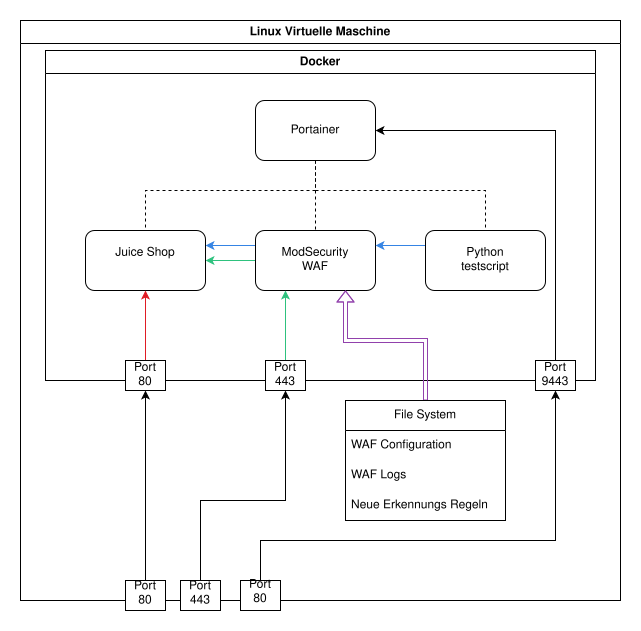
\includegraphics[width=0.9\textwidth]{./images/lab-setup.png}
    \caption{Aufbau der Laborumgebung}
    \floatfoot{Quelle: Eigene Darstellung}
    \label{fig:lab}
\end{figure}

Die Containervirtualisierungsumgebung Docker wird als Deployment-Umgebung verwendet.
Diese ermöglicht es, isolierte Ausführungsumgebungen für die Anwendungen zu erzeugen.
Der Aufbau dieser Umgebungen lässt sich mittels einer Konfigurationsdatei genau beschreiben und wiederholbar ausrollen.
Innerhalb der Umgebungen lassen sich virtuelle Netzwerke anlegen um Netzwerkkommunikation vom Host zu isolieren.
Dadurch lässt sich festlegen, wie und welche der einzelnen Anwendungen (Container) untereinander kommunizieren können.
Außerdem können Dateien oder Ordner aus dem Host-Dateisystem in den Container übergeben werden.
Dies ermöglicht es Konfigurationsdateien zur Verfügung zu stellen um die Container zu modifizieren, die sonst \textit{stateless} sind und nicht vorkonfiguriert ausgeliefert werden.
Im Gegensatz zu virtuellen Maschinen greift die Containervirtualisierungsumgebung direkt auf die Mittel des Host-Betriebssystem zu und benötigt dadurch deutlich weniger Rechenaufwand.\\

Wie in Abbildung \ref{fig:lab} dargestellt, werden in der Laborumgebung vier Container betrieben:

\begin{description}
    \item[ModSecurity \ac{waf}:] Der Hersteller, der in der Laborumgebung verwendeten \ac{waf}: \textit{ModSecurity}, stellt sein Produkt auch in Form eines Docker-Containers zur Verfügung. 
    Diese wird jedoch in modifizierter Form genutzt.
    Um die Lerninhalte zu vermittel muss die große Anzahl vorkonfigurierter Regeln, mit denen die \ac{waf} ausgeliefert wird um den Betrieb zu ermöglichen, entfernt werden.
    An dessen Stelle wird ein Verzeichnis aus dem Host-Dateisystem durchgereicht, in dem die Lernenden eigene Konfigurationen Platzieren können.
    Daneben werden, um das Debugging zu ermöglichen, die Log-Dateien aus der \ac{waf} im Host-Betriebssystem zur Verfügung gestellt.
    
    \item[Juice Shop:] Dieser wird in Version 16.0.0 verwendet, da der Hersteller (OWASP) die Anwendung regelmäßig verändert.
    Durch die Verwendung der neuesten Version könnten Challenges verloren gehen, die für die Durchführung der Aufgaben notwendig wäre.
    Auch diese Anwendung wird modifiziert.
    Es werden Daten hinterlegt und Nutzeraccounts angelegt.
    Diese ermöglichen es mittels eines automatischen Kontroll-Scripts die Konfiguration der \ac{waf} zu überprüfen.
    Im Rahmen der Thesis war es aus Zeitlichen Gründen nicht möglich das Kontroll-Script so fertigzustellen, dass es zuverlässig Ergebnisse liefert.

    \item[Python Test-Script:] Dieser Container enthält ein Python Skript, das es den Lernenden mittels des Unittest-Frameworks \textit{Pytest} ermöglicht, die erarbeiteten Lösungen zu überprüfen.
    Das Skript schickt \ac{http}-Requests durch die \ac{waf} und evaluiert die Antworten, um den Lernenden Rückmeldung über den Erfolg ihrer Konfiguration zu geben.
    Im Rahmen der Thesis war es aus Zeitlichen Gründen nicht möglich das Kontroll-Script so fertigzustellen, dass es zuverlässig Ergebnisse liefert.

    \item[Portainer:] Die Anwendung \textit{Portainer} ermöglicht es eine Docker Umgebung mittels einer grafischen Oberfläche zu verwalten.
    In der Laborumgebung kann sie genutzt werden um die Laborumgebung zu bedienen ohne sich tiefer mit der Funktion von Docker auseinander setzen zu müssen.
    Zwar können die Lernenden dies auch über das Docker Kommandozeilen-Interface tun, jedoch wird dies als eine vermeidbare Hürde betrachtet, die den Einstieg erschweren könnte.
    Die grafische Oberfläche soll unter anderem genutzt werden um den \ac{waf}-Container nach einer Konfigurationsänderung neu zu starten und mit dem Test Skript zu interagieren. 
\end{description}

Aus den oben genannten Containern ergibt sich eine Netzwerk-Architektur innerhalb der Umgebung, die entsprechend aufgebaut werden muss.
So ist es notwendig, dass eine Verbindung von dem Python-Test-Container zur \ac{waf} und von dieser zum Juice Shop aufgebaut werden kann.
Hierfür werden separate Docker-Netzwerke erstellt die an den Containern angeschlossen sind.
Um den Nutzern eine Interaktion mit den Containern zu ermöglichen werden einige Ports aus der Docker-Umgebung freigegeben:

\begin{itemize}
    \item Die ungesicherte Weboberfläche des Juice Shops (Port 80 [\ac{http}])
    \item Die, durch die \ac{waf} gesicherte, Weboberfläche des Juice Shops (Port 443 [\ac{https}])
    \item Das Management Interface der Portainer-Anwendung (Port 9443 [\ac{https}])
\end{itemize}

Durch die oben beschriebene Docker Umgebung sind Anforderungen an die Laborumgebung wie dem \textit{einheitlichen Deployment} und der \textit{Modifizierbarkeit der Anwendungen} bereits erfüllt.
Es ergeben sich jedoch auch einige Herausforderungen:

\begin{itemize}
    \item Docker ist zwar als Cross-Platform Anwendung konzipiert.
    Es stehen Versionen für die drei gängigen Betriebssysteme Windows, MacOS und Linux zur Verfügung.
    Jedoch bauen die verwendeten Container hauptsächlich auf Linux auf.
    In der Theorie sollte dies zu keinen Problemen führen, da Docker in der Lage ist nicht Platform-Native Container auf sich unterscheidenden Betriebssystemen auszuführen, jedoch kann ein solcher Aufbau durchaus zu unvorhergesehenen Problemen führen.
    \item Ein weiteres Problem ist, dass durch das Durchreichen von Dateien zwischen Container und dem Host-Dateisystem zusätzlicher Konfigurationsaufwand für die Nutzer entsteht.
\end{itemize}

Um diese Probleme zu mitigieren wird die Laborumgebung als Linux Virtuelle Maschine ausgeliefert.
In dieser ist eine Docker-Umgebung vorinstalliert und die Container und Netzwerke bereits präsent und werde automatisiert gestartet.
Dies ermöglicht die Auslieferung mittels einer \ac{vm}-Datei, in der die Konfigurationen schon an einer einheitlichen Stelle enthalten sind.
Lernende müssen zur Nutzung also nur eine virtuelle Maschinen auf ihren Rechnern importieren und mittels eines virtuellen Netzwerk Interface auf die Weboberflächen zugreifen.
Die Konfiguration der \ac{waf} findet in Textdateien statt, die sich in der Virtuellen Maschine befinden.
Der Zugriff auf diese ist mit dem Text-Editor Visual Studio Code der Firma Microsoft vorgesehen, da dieser eine SSH Erweiterung hat die es mit geringen Konfigurationsaufwand ermöglicht Dateien auf entfernten Servern oder in \acp{vm} zu bearbeiten.

Die Nutzung der Laborumgebung werden durch diese Maßnahmen als einfach genug beurteilt um einen schnellen Einstieg zu ermöglichen.
Die Konfigurationen, die vorgenommen werden müssen, werden in der ersten Lerneinheit (Kapitel \ref{sec:learning-unit-1}) beschrieben.
Es steht den Lernenden frei weitere oder andere als die beschriebenen Technologien zu verwenden, um mit der Laborumgebung zu interagieren.
Diese können im Rahmen dieser Thesis und den Aufgabenstellungen jedoch nicht berücksichtigt werden.

\pagebreak